% Created by tikzDevice version 0.10.1 on 2018-01-31 10:28:43
% !TEX encoding = UTF-8 Unicode
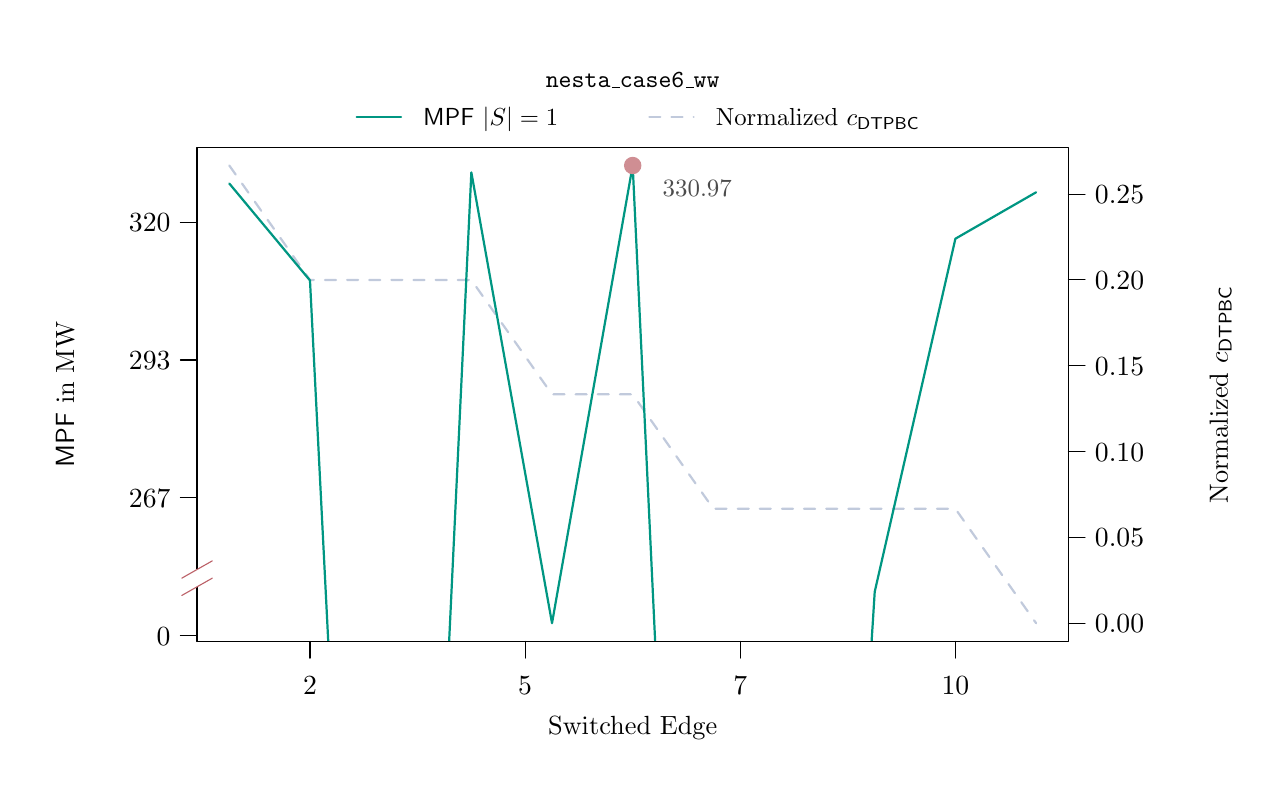
\begin{tikzpicture}[x=1pt,y=1pt]
\definecolor{fillColor}{RGB}{255,255,255}
\path[use as bounding box,fill=fillColor,fill opacity=0.00] (0,0) rectangle (440.85,271.01);
\begin{scope}
\path[clip] (  0.00,  0.00) rectangle (440.85,271.01);
\definecolor{drawColor}{RGB}{193,202,220}

\path[draw=drawColor,line width= 0.8pt,dash pattern=on 4pt off 4pt ,line join=round,line cap=round] ( 72.86,221.20) --
	(102.01,179.85) --
	(131.17,179.85) --
	(160.32,179.85) --
	(189.47,138.51) --
	(218.62,138.51) --
	(247.78, 97.16) --
	(276.93, 97.16) --
	(306.08, 97.16) --
	(335.23, 97.16) --
	(364.39, 55.82);
\end{scope}
\begin{scope}
\path[clip] (  0.00,  0.00) rectangle (440.85,271.01);
\definecolor{drawColor}{RGB}{0,0,0}

\path[draw=drawColor,line width= 0.4pt,line join=round,line cap=round] ( 61.20, 49.20) --
	(376.05, 49.20) --
	(376.05,227.81) --
	( 61.20,227.81) --
	( 61.20, 49.20);
\end{scope}
\begin{scope}
\path[clip] (  0.00,  0.00) rectangle (440.85,271.01);
\definecolor{drawColor}{RGB}{0,0,0}

\path[draw=drawColor,line width= 0.4pt,line join=round,line cap=round] (376.05, 55.82) -- (376.05,210.86);

\path[draw=drawColor,line width= 0.4pt,line join=round,line cap=round] (376.05, 55.82) -- (382.05, 55.82);

\path[draw=drawColor,line width= 0.4pt,line join=round,line cap=round] (376.05, 86.82) -- (382.05, 86.82);

\path[draw=drawColor,line width= 0.4pt,line join=round,line cap=round] (376.05,117.83) -- (382.05,117.83);

\path[draw=drawColor,line width= 0.4pt,line join=round,line cap=round] (376.05,148.84) -- (382.05,148.84);

\path[draw=drawColor,line width= 0.4pt,line join=round,line cap=round] (376.05,179.85) -- (382.05,179.85);

\path[draw=drawColor,line width= 0.4pt,line join=round,line cap=round] (376.05,210.86) -- (382.05,210.86);

\node[text=drawColor,anchor=base west,inner sep=0pt, outer sep=0pt, scale=  1.00] at (385.65, 52.37) {0.00};

\node[text=drawColor,anchor=base west,inner sep=0pt, outer sep=0pt, scale=  1.00] at (385.65, 83.38) {0.05};

\node[text=drawColor,anchor=base west,inner sep=0pt, outer sep=0pt, scale=  1.00] at (385.65,114.39) {0.10};

\node[text=drawColor,anchor=base west,inner sep=0pt, outer sep=0pt, scale=  1.00] at (385.65,145.40) {0.15};

\node[text=drawColor,anchor=base west,inner sep=0pt, outer sep=0pt, scale=  1.00] at (385.65,176.41) {0.20};

\node[text=drawColor,anchor=base west,inner sep=0pt, outer sep=0pt, scale=  1.00] at (385.65,207.42) {0.25};
\end{scope}
\begin{scope}
\path[clip] (  0.00,  0.00) rectangle (440.85,271.01);
\definecolor{drawColor}{RGB}{0,150,130}

\path[draw=drawColor,line width= 0.8pt,line join=round,line cap=round] (118.89,238.60) -- (134.91,238.60);
\definecolor{drawColor}{RGB}{193,202,220}

\path[draw=drawColor,line width= 0.8pt,dash pattern=on 4pt off 4pt ,line join=round,line cap=round] (224.63,238.60) -- (240.65,238.60);
\definecolor{drawColor}{RGB}{0,0,0}

\node[text=drawColor,anchor=base,inner sep=0pt, outer sep=0pt, scale=  0.89] at (218.62,249.28) {\texttt{nesta\_case6\_ww}};

\node[text=drawColor,anchor=base west,inner sep=0pt, outer sep=0pt, scale=  0.89] at (142.92,235.54) {$\mathsf{MPF}~|S|=1$};

\node[text=drawColor,anchor=base west,inner sep=0pt, outer sep=0pt, scale=  0.89] at (248.66,235.54) {Normalized~$c_\mathsf{DTPBC}$};
\end{scope}
\begin{scope}
\path[clip] (  0.00,  0.00) rectangle (440.85,271.01);
\definecolor{drawColor}{RGB}{0,0,0}

\path[draw=drawColor,line width= 0.4pt,line join=round,line cap=round] ( 61.20, 51.35) -- ( 61.20,200.71);

\path[draw=drawColor,line width= 0.4pt,line join=round,line cap=round] ( 61.20, 51.35) -- ( 55.20, 51.35);

\path[draw=drawColor,line width= 0.4pt,line join=round,line cap=round] ( 61.20,101.13) -- ( 55.20,101.13);

\path[draw=drawColor,line width= 0.4pt,line join=round,line cap=round] ( 61.20,150.92) -- ( 55.20,150.92);

\path[draw=drawColor,line width= 0.4pt,line join=round,line cap=round] ( 61.20,200.71) -- ( 55.20,200.71);

\node[text=drawColor,anchor=base east,inner sep=0pt, outer sep=0pt, scale=  1.00] at ( 51.60, 47.90) {0};

\node[text=drawColor,anchor=base east,inner sep=0pt, outer sep=0pt, scale=  1.00] at ( 51.60, 97.69) {267};

\node[text=drawColor,anchor=base east,inner sep=0pt, outer sep=0pt, scale=  1.00] at ( 51.60,147.48) {293};

\node[text=drawColor,anchor=base east,inner sep=0pt, outer sep=0pt, scale=  1.00] at ( 51.60,197.26) {320};
\end{scope}
\begin{scope}
\path[clip] (  0.00,  0.00) rectangle (440.85,271.01);
\definecolor{drawColor}{RGB}{255,255,255}
\definecolor{fillColor}{RGB}{255,255,255}

\path[draw=drawColor,line width= 0.4pt,line join=round,line cap=round,fill=fillColor] ( 55.69, 68.96) rectangle ( 66.71, 75.22);
\definecolor{drawColor}{RGB}{188,97,104}

\path[draw=drawColor,line width= 0.4pt,line join=round,line cap=round] ( 55.69, 65.84) -- ( 66.71, 72.09);

\path[draw=drawColor,line width= 0.4pt,line join=round,line cap=round] ( 55.69, 72.09) -- ( 66.71, 78.34);
\end{scope}
\begin{scope}
\path[clip] ( 61.20, 49.20) rectangle (376.05,227.81);
\definecolor{drawColor}{RGB}{0,150,130}

\path[draw=drawColor,line width= 0.8pt,line join=round,line cap=round] ( 72.86,214.69) --
	(102.01,179.67) --
	(111.10,  0.00);

\path[draw=drawColor,line width= 0.8pt,line join=round,line cap=round] (149.96,  0.00) --
	(160.32,218.72) --
	(189.47, 55.82) --
	(218.62,221.20) --
	(229.06,  0.00);

\path[draw=drawColor,line width= 0.8pt,line join=round,line cap=round] (301.86,  0.00) --
	(306.08, 67.19) --
	(335.23,194.75) --
	(364.39,211.52);
\end{scope}
\begin{scope}
\path[clip] ( 61.20, 49.20) rectangle (376.05,227.81);
\definecolor{fillColor}{RGB}{207,142,147}

\path[fill=fillColor] (218.62,221.20) circle (  3.15);
\end{scope}
\begin{scope}
\path[clip] ( 61.20, 49.20) rectangle (376.05,227.81);
\definecolor{drawColor}{gray}{0.30}

\node[text=drawColor,anchor=base,inner sep=0pt, outer sep=0pt, scale=  0.90] at (241.95,210.04) {330.97};
\end{scope}
\begin{scope}
\path[clip] (  0.00,  0.00) rectangle (440.85,271.01);
\definecolor{drawColor}{RGB}{0,0,0}

\path[draw=drawColor,line width= 0.4pt,line join=round,line cap=round] (102.01, 49.20) -- (335.23, 49.20);

\path[draw=drawColor,line width= 0.4pt,line join=round,line cap=round] (102.01, 49.20) -- (102.01, 43.20);

\path[draw=drawColor,line width= 0.4pt,line join=round,line cap=round] (179.75, 49.20) -- (179.75, 43.20);

\path[draw=drawColor,line width= 0.4pt,line join=round,line cap=round] (257.49, 49.20) -- (257.49, 43.20);

\path[draw=drawColor,line width= 0.4pt,line join=round,line cap=round] (335.23, 49.20) -- (335.23, 43.20);

\node[text=drawColor,anchor=base,inner sep=0pt, outer sep=0pt, scale=  1.00] at (102.01, 30.00) {2};

\node[text=drawColor,anchor=base,inner sep=0pt, outer sep=0pt, scale=  1.00] at (179.75, 30.00) {5};

\node[text=drawColor,anchor=base,inner sep=0pt, outer sep=0pt, scale=  1.00] at (257.49, 30.00) {7};

\node[text=drawColor,anchor=base,inner sep=0pt, outer sep=0pt, scale=  1.00] at (335.23, 30.00) {10};

\node[text=drawColor,anchor=base,inner sep=0pt, outer sep=0pt, scale=  0.95] at (218.62, 15.60) {Switched Edge};

\node[text=drawColor,rotate= 90.00,anchor=base,inner sep=0pt, outer sep=0pt, scale=  0.95] at ( 16.80,138.51) {$\mathsf{MPF}$ in~$\mathrm{MW}$};

\node[text=drawColor,rotate= 90.00,anchor=base,inner sep=0pt, outer sep=0pt, scale=  0.95] at (433.65,138.51) {Normalized~$c_\mathsf{DTPBC}$};
\end{scope}
\end{tikzpicture}
